\documentclass[notes,slidesec,a4]{seminar}
\usepackage[latin1]{inputenc}

\usepackage{t-gsyc-6}
\usepackage{fancybox}
\usepackage{graphics}
\usepackage{moreverb}
\usepackage{alltt}
\usepackage{html}
\usepackage{hthtml}
\usepackage{color}
\usepackage[usenames,dvipsnames,svgnames,table]{xcolor}
\usepackage{amsmath}
\usepackage[normalsize]{subfigure}
\usepackage{url}
\usepackage{hyperref}
\usepackage{listings}
\usepackage{multirow}
%\date{}

\title{WEB TECHNOLOGIES IN JDEROBOT FRAMEWORK 
%\\ \vspace{0.2cm} 
 FOR ROBOTICS}
\author{Aitor Mart�nez Fern�ndez
\\Jose Maria Ca�as Plaza}
%\coauthor{Jose Maria Ca�as Plaza}

\cop{Aitor Mart�nez Fern�ndez}
\address{josemaria.plaza@urjc.es}

\begin{document}
\maketitle

%%--------------------------------------------------------------

\begin{hslide}
\slsect{Index}
\begin{itemize}
\item Introduction 
\item JdeRobot
\item Web Tools
\item Experiments
\item Conclusions
\end{itemize}
\end{hslide}

%%--------------------------------------------------------------
\begin{hslide}
\slsect{Introduction}
In the last years, several robotic frameworks (SDKs) 
have appeared that simplify and speed up the development of robot applications.

The SDKs facilitate access to the sensors and actuators of the robots.
\begin{minipage}[t]{0.5\textwidth}
\begin{figure}[htb]
\centering
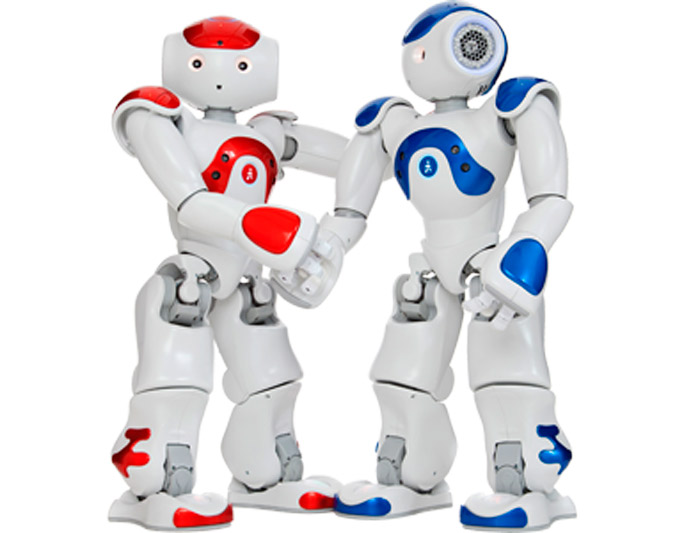
\includegraphics[width=0.8\textwidth]{img/nao.jpg}
\end{figure}
\end{minipage}
\begin{minipage}[t]{0.5\textwidth}
\begin{figure}[htb]
\centering
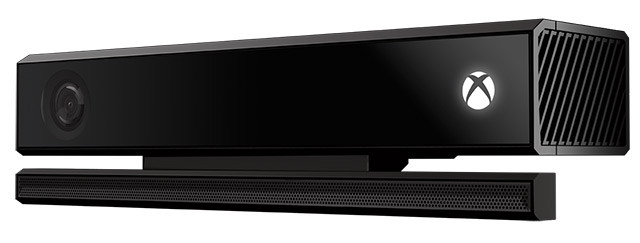
\includegraphics[width=0.5\textwidth]{img/kinect2.jpg}
\end{figure}
\hspace{1cm}
\begin{figure}[htb]
\centering
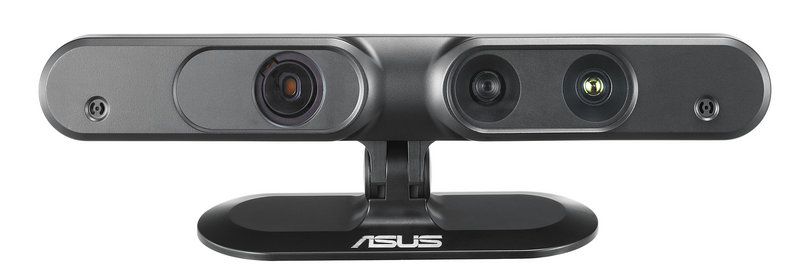
\includegraphics[width=0.5\textwidth]{img/xtion.jpg}
\end{figure}
%\begin{figure}[htb]
%\centering
%\subfigure[]{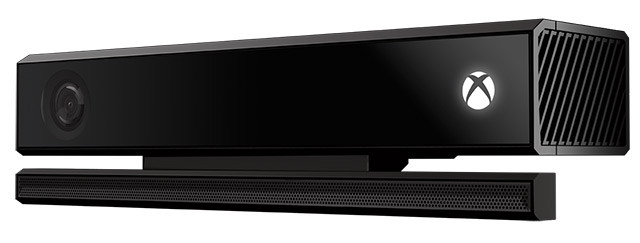
\includegraphics[width=0.5\textwidth]{img/kinect2.jpg}}
%\hspace{1cm}
%\subfigure[]{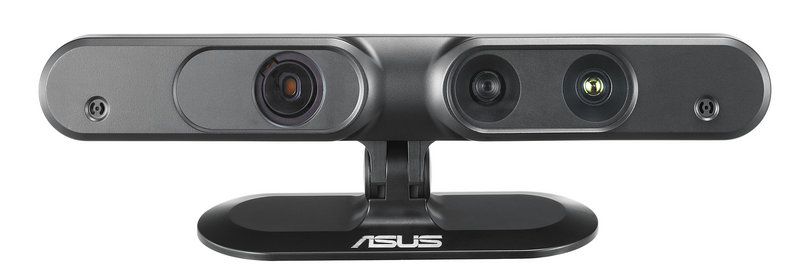
\includegraphics[width=0.5\textwidth]{img/xtion.jpg}}
%\end{figure}
\end{minipage}
\end{hslide}


%%--------------------------------------------------------------
%\begin{hslide}
%\slsubsect{Antecedentes}
%\begin{itemize}
%\item JdeRobot: Es una plataforma de desarrollo de aplicaciones orientadas a la rob�tica,
%dom�tica y visi�n artificial desarrollada por el grupo de Rob�tica de la URJC.
%\item ICE: Permite comunicaciones cross-language y cross-platform.
%\end{hslide}

%%--------------------------------------------------------------

\begin{hslide}
\slsect{JdeRobot}

\begin{itemize}
\item Provides a distributed component-based programming environment.
\item Components may be written in C++, Python, Java, JavaScript...
\item Uses ICE: Allows cross-language and cross-platform communications.
\item currently supports Cameras, RGBD sensors, Kobuki, ArDrone,...
\end{itemize}
\begin{minipage}[t]{0.5\textwidth}
\begin{figure}[htb]
\centering
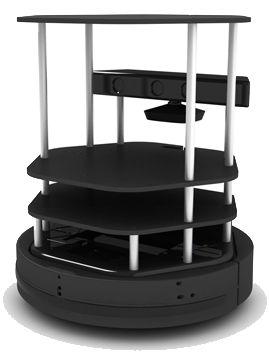
\includegraphics[width=0.4\textwidth]{img/turtlebot_2_lg.png}
\end{figure}
\end{minipage}
\begin{minipage}[t]{0.5\textwidth}
\begin{figure}[htb]
\centering
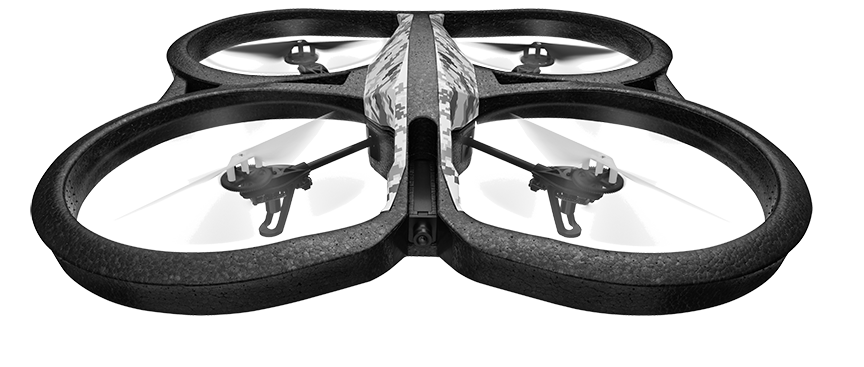
\includegraphics[width=\textwidth]{img/ardrone.png}
\end{figure}
\end{minipage}
\end{hslide}


%%---------------------------------------------------------------

\begin{hslide}
\slsect{Web Tools}
Web tools have been developed using last generation web technologies like HTML5, JavaScript, CSS, WebGL, WebWorkers and WebSockets.
\begin{center}
\begin{figure}
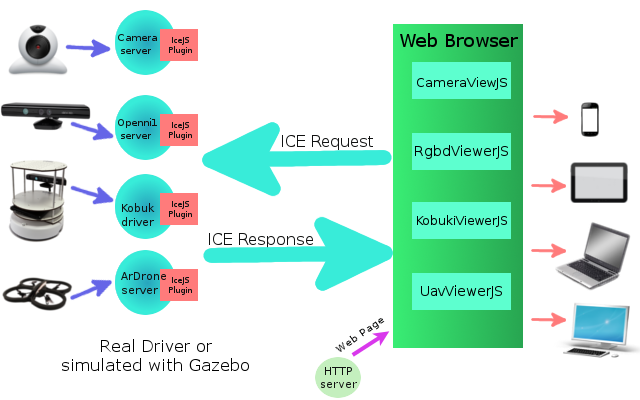
\includegraphics[width=0.75\textwidth]{img/esquema_ingles.png}
\end{figure}
\end{center}  
\end{hslide}

%%---------------------------------------------------------------
\begin{hslide}
\slsubsect{CameraViewJS}
\begin{minipage}{6cm}
\begin{itemize}
 \item When it is run, the widgets are initiated, creates the \textit{WebWorker} and starts the stream.
 \item The \texttt{connect} function establishes a JavaScript promise that is resolved when the WebWorker indicates that the connection has been established. 
 \item It constantly requests sensor data to the driver and passes them to the main thread.
\end{itemize}
\end{minipage} \hfill
\begin{minipage}{6cm}
\begin{center}
\begin{figure}
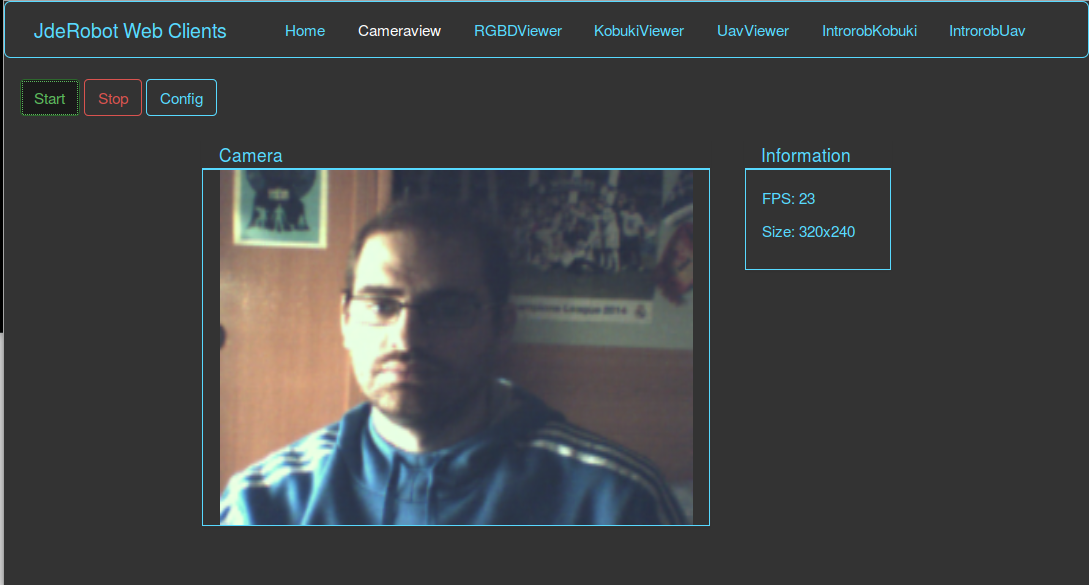
\includegraphics[width=5cm]{img/jrwc_cameraview.png}
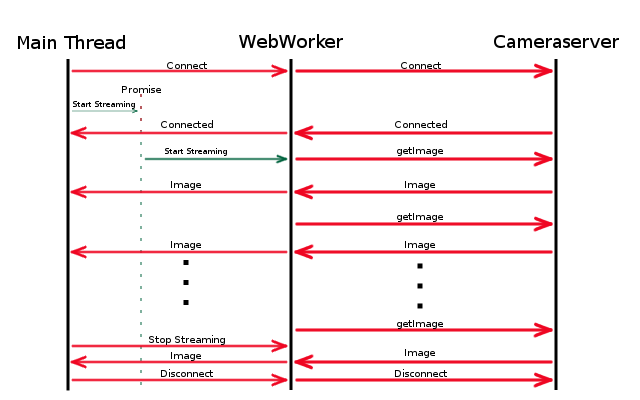
\includegraphics[width=5.6cm]{img/mensajes_cameraview_ingles.png}
\end{figure}
\end{center}
\end{minipage}
\end{hslide}

%%---------------------------------------------------------------
%\begin{hslide}
%\slsubsect{CameraViewJS}
%\begin{minipage}{6cm}
%\begin{center}
%\begin{figure}
%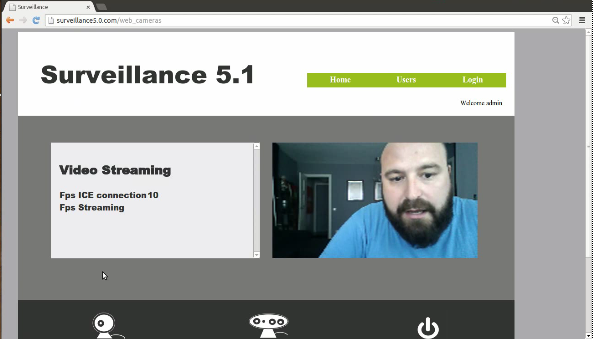
\includegraphics[width=5cm]{img/surveillance5.png}
%\end{figure}
%\end{center}
%\begin{enumerate}
% \setcounter{enumi}{2}
% \item Se inicia el Streaming de video
%\item Cada vez que se recibe una imagen se muestra en el canvas
%\end{enumerate}
%\end{minipage} \hfill
%\begin{minipage}{6cm}

%\begin{enumerate}
%\item Se incian los widgets y se crean los WebWorkers
%\item Mediante una promesa se espera a tener establecida la conexi�n con el servidor
%\end{enumerate}
%\begin{center}
%\begin{figure}
%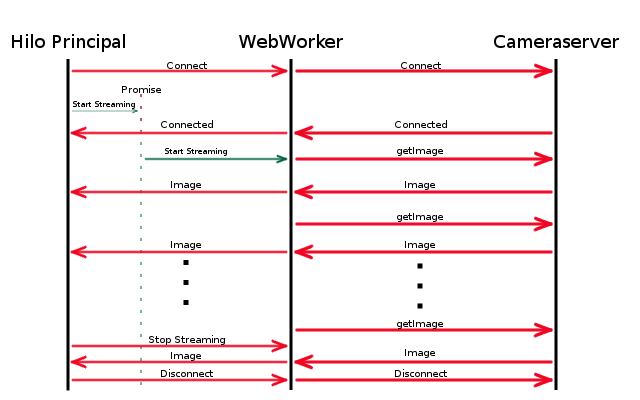
\includegraphics[width=5.9cm]{img/mensajes_cameraview.png}
%\end{figure}
%\end{center}
%\end{minipage}
%\end{hslide}

%%---------------------------------------------------------------
\begin{hslide}
\slsubsect{RgbdViewerJS}
\begin{itemize}
\item Images like in CameraViewJS. 
\item When two camera images have been received, creates the 3D point cloud and shown in the 3D model.
\end{itemize}
\begin{center}
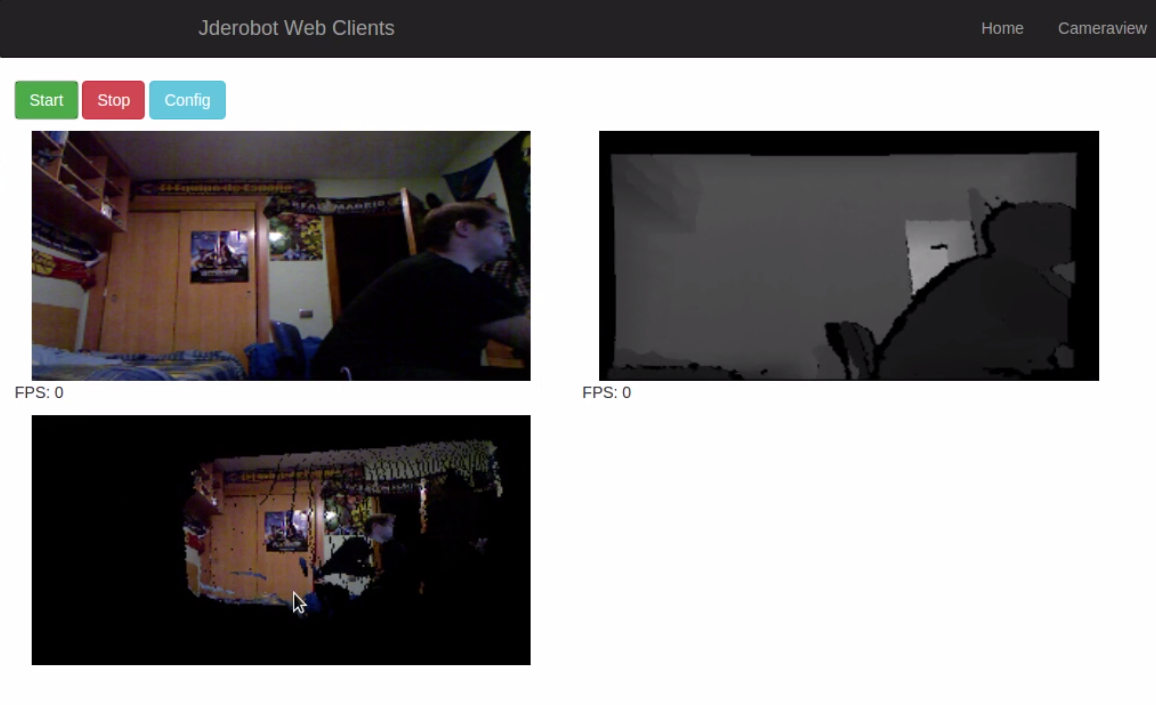
\includegraphics[width=0.7\textwidth]{img/rgbdviewer.png}
\end{center}
\end{hslide}

%%---------------------------------------------------------------
\begin{hslide}
\slsubsect{KobukiViewerJS}
\begin{minipage}{5cm}
\begin{center}
\begin{figure}
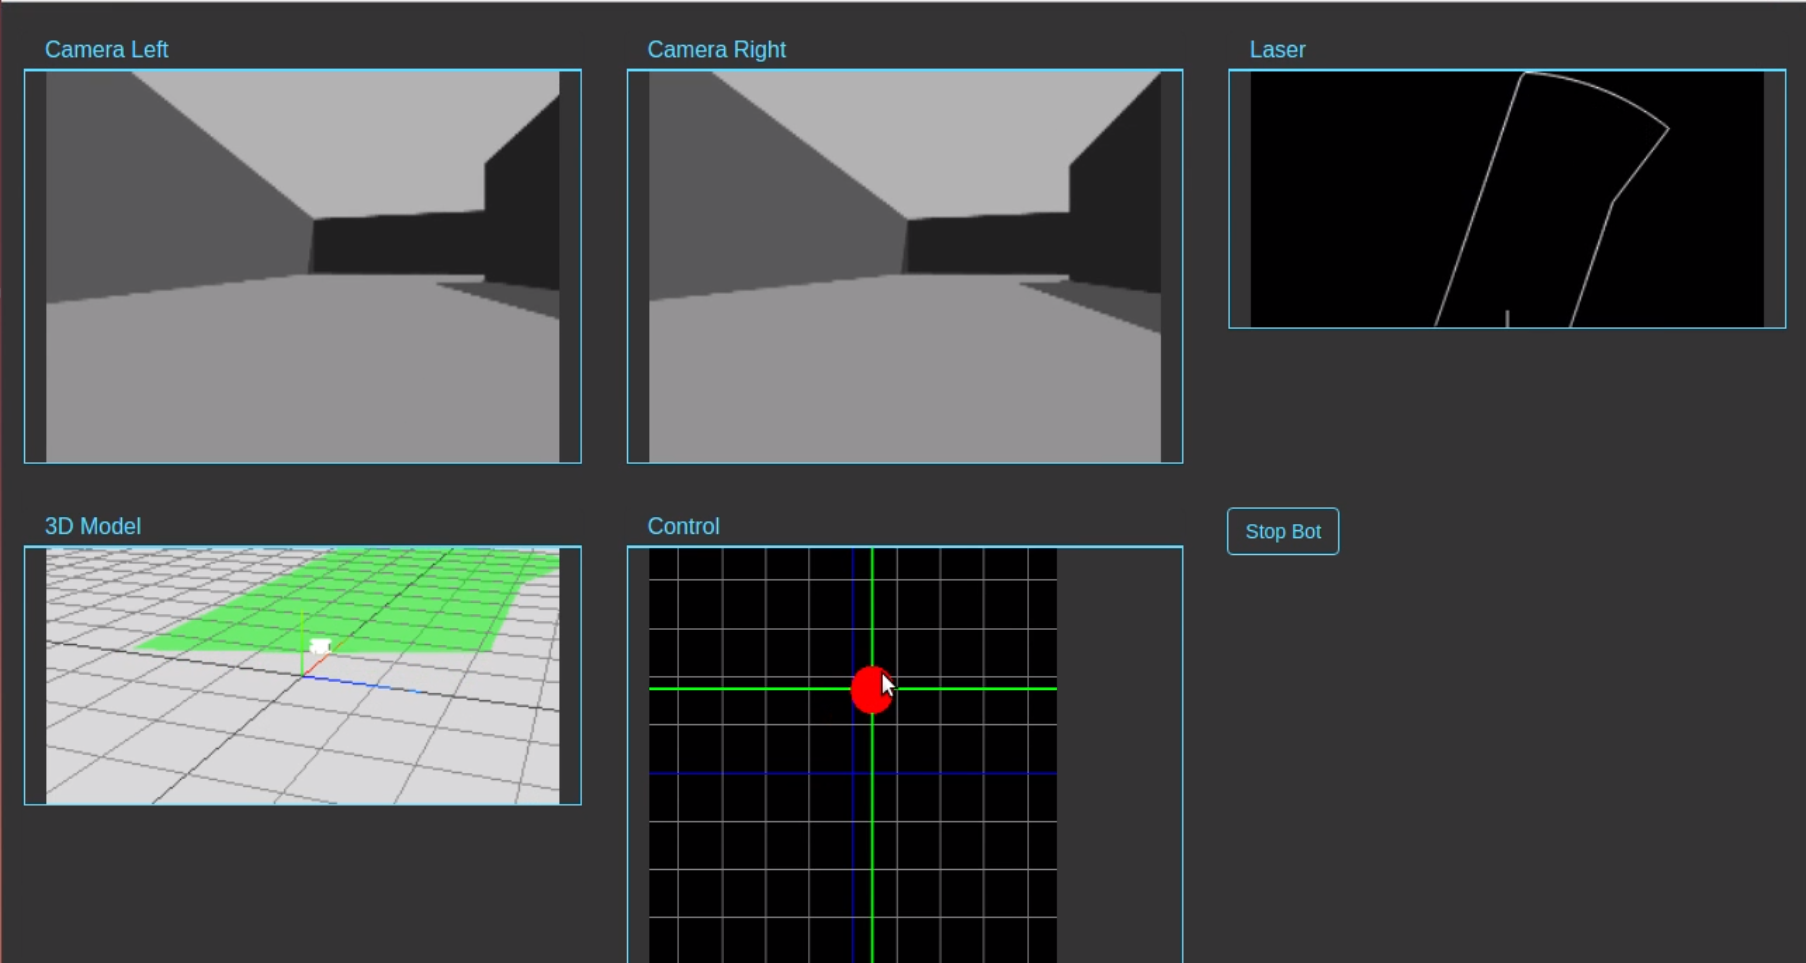
\includegraphics[width=5cm]{img/kobukiviewer_body.png}
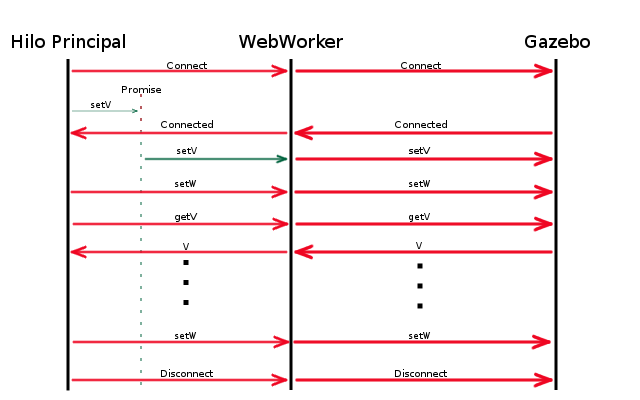
\includegraphics[width=5cm]{./img/mensajes_motors.png}
\end{figure}
\end{center}
\end{minipage} \hfill
\begin{minipage}{6cm}
\begin{itemize}
\item Images like in CameraViewJS.
\item Whenever it receives a Pose3D, modifies the position and orientation of the robot in the 3D model.
\item When it receives information from laser, creates a 2D and other 3D image.
\item Whenever you move the control speed orders are sended.
\end{itemize}
\end{minipage}
\end{hslide}

\begin{hslide}
\slsubsect{UavViewerJS}
\begin{minipage}{5cm}
\begin{center}
\begin{figure}
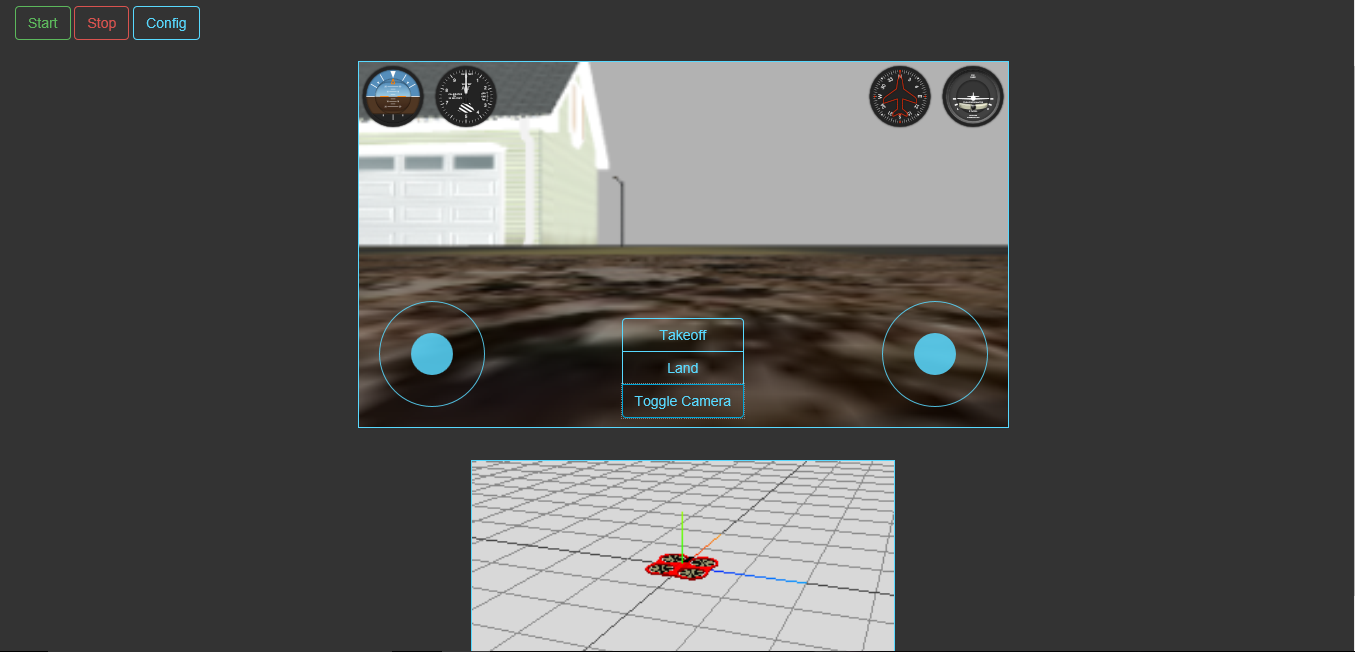
\includegraphics[width=\textwidth]{img/body_uavviewer2.png}
\end{figure}
\end{center}
\end{minipage} \hfill
\begin{minipage}{6cm}
\begin{itemize}
\item Images like in CameraViewJS.
\item Whenever it receives a Pose3D, modifies the position and orientation of the drone in the 3D model and flight indicators are modified.
\item Whenever the controls move, speed orders are sent to the drone.
\item When the buttons are pressed, take off, landing,... orders are sent to the drone
\end{itemize}
\end{minipage}
\end{hslide}


%%---------------------------------------------------------------
\begin{hslide}
\slsect{Experiments}
\begin{itemize}
\item CameraViewJS.
\item RgbdViewerJS.
\item KobukiViewerJS.
\item UavViewerJS.
\item Framerate.
\end{itemize}
\end{hslide}


%%---------------------------------------------------------------
\begin{hslide}
\slsubsect{Framerate}
 \begin{table}[]
\centering
{\tiny
\begin{tabular}{|
>{\columncolor[HTML]{67FD9A}}c |
>{\columncolor[HTML]{9AFF99}}c |
>{\columncolor[HTML]{34CDF9}}c |
>{\columncolor[HTML]{38FFF8}}c |
>{\columncolor[HTML]{96FFFB}}c |
>{\columncolor[HTML]{FFCE93}}c |
>{\columncolor[HTML]{FFFC9E}}c |}
\hline
\multicolumn{2}{|c|}{\cellcolor[HTML]{32CB00}\textbf{CameraServer}}                                                          & \multicolumn{3}{c|}{\cellcolor[HTML]{3166FF}\textbf{Clientes}}                                                                              & \cellcolor[HTML]{FFCE93}                                                                                    & \cellcolor[HTML]{FFFFC7}                                                                                      \\ \cline{1-5}
\textbf{Location}                                   & \textbf{\begin{tabular}[c]{@{}c@{}}Mbps\\ down/up\end{tabular}} & \textbf{Kind} & \textbf{Location}                                  & \textbf{\begin{tabular}[c]{@{}c@{}}Mbps\\ down/up\end{tabular}} & \multirow{-2}{*}{\cellcolor[HTML]{FFCE93}\textbf{\begin{tabular}[c]{@{}c@{}}FPS\\ CameraView\end{tabular}}} & \multirow{-2}{*}{\cellcolor[HTML]{FFFFC7}\textbf{\begin{tabular}[c]{@{}c@{}}FPS\\ CameraViewJS\end{tabular}}} \\ \hline
\begin{tabular}[c]{@{}c@{}}Same\\ PC\end{tabular}   & -                                                                     & PC            & \begin{tabular}[c]{@{}c@{}}Same\\ PC\end{tabular}  & -                                                                     & 9                                                                                                           & 8                                                                                                             \\ \hline
\begin{tabular}[c]{@{}c@{}}Local\\ network\end{tabular}  & 1000/1000                                                             & PC            & \begin{tabular}[c]{@{}c@{}}Local\\ network\end{tabular} & 65/65                                                                 & 6                                                                                                           & 4                                                                                                             \\ \hline
\begin{tabular}[c]{@{}c@{}}Local\\ network\end{tabular}  & 1000/1000                                                             & Mobile         & \begin{tabular}[c]{@{}c@{}}Local\\ network\end{tabular} & 65/65                                                                 & -                                                                                                           & 4                                                                                                             \\ \hline
Home                                                 & 50/5                                                                  & PC            & URJC                                                & 15/15                                                                 & 1                                                                                                           & 1                                                                                                             \\ \hline
Home                                                 & 50/5                                                                  & Mobile         & 3G                                                  & 5/1                                                                   & -                                                                                                           & 1                                                                                                             \\ \hline
Home                                                 & 50/5                                                                  & Mobile         & 4G                                                  & 13/4                                                                  & -                                                                                                           & 1                                                                                                             \\ \hline
URJC                                                 & 100/100                                                               & PC            & Home                                                & 50/5                                                                  & 6                                                                                                           & 4                                                                                                             \\ \hline
URJC                                                 & 100/100                                                               & Mobile         & 3G                                                  & 5/1                                                                   & -                                                                                                           & 2                                                                                                             \\ \hline
URJC                                                 & 100/100                                                               & Mobile         & 4G                                                  & 13/4                                                                  & -                                                                                                           & 4                                                                                                           \\ \hline
\end{tabular}
}
\end{table}

\end{hslide}

%%---------------------------------------------------------------
\begin{hslide}
\slsect{Conclusions}
\begin{itemize}
\item Four webtools have been created in JdeRobot that allow to teleoperate wheeled robots or drones and to monitor cameras and RGBD sensors from any browser.
\item Multitplatform and multi-device
\item They use advanced web technologies like WebSockets, WebGL and WebWorkers
\end{itemize}
\end{hslide}

\end{document}
